\documentclass[a4paper,UTF8]{ctexart}

\usepackage{amsmath, amsthm, amssymb, amsfonts, hyperref, mathrsfs}%美国数学学会的包+?
\usepackage{geometry} %控制界面
\usepackage{bookmark}
\usepackage{fancyhdr} % header & footer
\usepackage{appendix} % 附录
\usepackage{tikz} %作图
\usepackage{graphicx} %插入图片的宏包
\usepackage{float} %设置图片浮动位置的宏包
%\usepackage{subfigure} %插入多图时用子图显示的宏包
\usepackage{listings} %引用代码
\usepackage{physics,mathtools} %物理数学工具
\usepackage{comment}
\usepackage{framed}
\usepackage{caption}
\usepackage{subcaption}
\geometry{top=2.5cm,bottom=2.5cm,left=2.5cm,right=2.5cm} % 布局要求
\pagestyle{fancy} % fancy分格
\fancyhf{} % 清除所有页眉页脚
\renewcommand\headrulewidth{0.6pt}
\renewcommand\footrulewidth{0.6pt}
% font
\setCJKmainfont{Noto Serif CJK SC}[BoldFont={Noto Serif CJK SC Bold}, ItalicFont=]
\lhead{何金铭 PB21020660$\mid$座位号:3}
\chead{慢中子探测预习报告}
\rhead{\thepage}
\lfoot{2024.4.7}
\rfoot{USTC}
%\bibliographystyle{plain} % 引用样式
\everymath{\displaystyle} % display
%============================================================

\begin{document}

\begin{center}
    \textbf{\Large 慢中子探测预习报告}
    \par \text{\large 何金铭 PB21020660}
\end{center}

\section{实验目的}

\begin{enumerate}
    \item 了解核反应法测量中子的原理。
    \item 学习选取$BF_3$正比计数管测量慢中子工作条件的方法。
\end{enumerate}

\section{实验原理}

\subsection{$BF_3$正比计数管}

$BF_3$正比计数管是充三氟化硼气体、工作在气体放大正比区的慢中子探测器:由于$^{10}B(n,\alpha)$截面随中子能量变化在$E_n < 30keV$时有“速度反比”关系,即

\begin{equation}
    \sigma(E) \propto \frac{1}{v} \propto \frac{1}{\sqrt{E_n}}
\end{equation}

故$BF_3$正比计数管是对热中子为主的慢中子灵敏(热中子截面为3840b)。
它所需要的设备简单,测量稳定可靠,能甄别中子和$\gamma$射线,
附设慢化体后还可以用来探测快中子。例如,用$BF_3$正比计数管加石蜡或聚乙烯做成的“长计数管”就是一种很常用的快中子通量监测器;
这儿“长计数管”是起名于可以在很宽的中子能量范围内对快中子响应灵敏度基本不变。

\subsection{$BF_3$正比计数管探测中子的脉冲幅度谱}

下图给出了给出了一个典型的$BF_3$正比计数管输出的脉冲幅度谱:

\begin{figure}[H]
    \centering
    \begin{minipage}[b]{0.9\textwidth}
        \centering
        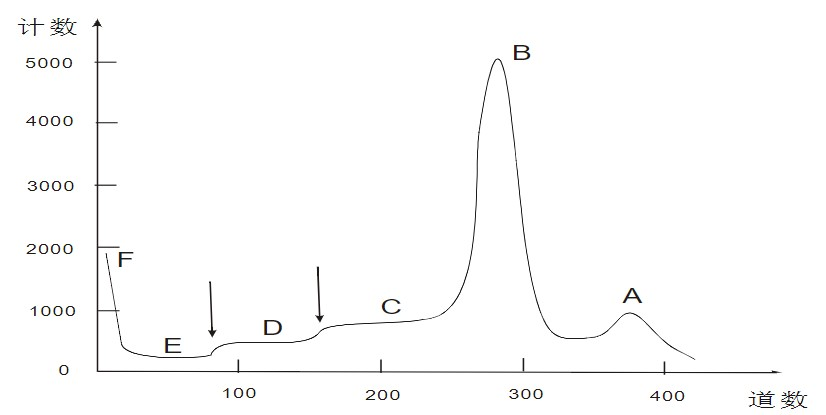
\includegraphics[width=0.9\textwidth]{./fig1.jpg}
        \caption{$BF_3$正比计数管的脉冲幅度谱}
    \end{minipage}
\end{figure}

图中有几个典型的以下区域:

\begin{itemize}
    \item 峰A:对应$6\%$分支,$^{10}B + n \rightarrow ^{7}Li + \alpha + 2.79MeV $
    \item 峰B:对应$94\%$分支,$^{10}B + n \rightarrow ^{7}Li^{\star} + \alpha + 2.31MeV $,$^{7}Li^{\star} \rightarrow ^{7}Li + \gamma(0.48MeV)$
    \item 平台区C,由于核反应发生在计数管近壁区的壁效应所致
    \item 平台区D,由于核反应发生在计数管近壁区的壁效应所致
    \item 平坦低谷区E,由于核反应发生在计数管近壁区的壁效应所致
    \item 平坦低谷区F,是由于探测器噪声和射线在管内转换成的电子产生的低幅度事件造成的(对于噪声水平高的前级放大器的探测系统,F区还包含着电子学噪声).
    但$BF_3$正比计数管用简单的幅度甄别方法可以方便地将$\gamma$本底去掉
\end{itemize}

\subsection{$BF_3$正比计数管的高压坪曲线和甄别阈曲线}

高压坪曲线是探测器计数系统的甄别阈固定时,计数率随高压变化的关系曲线。
甄别阈曲线是高压固定时,计数率随甄别阈改变的关系曲线。
探测器的脉冲幅度谱决定了甄别阈曲线及高压坪曲线的形状,如下图所示。

\begin{figure}[H]
    \centering
    \begin{minipage}[b]{1\textwidth}
        \centering
        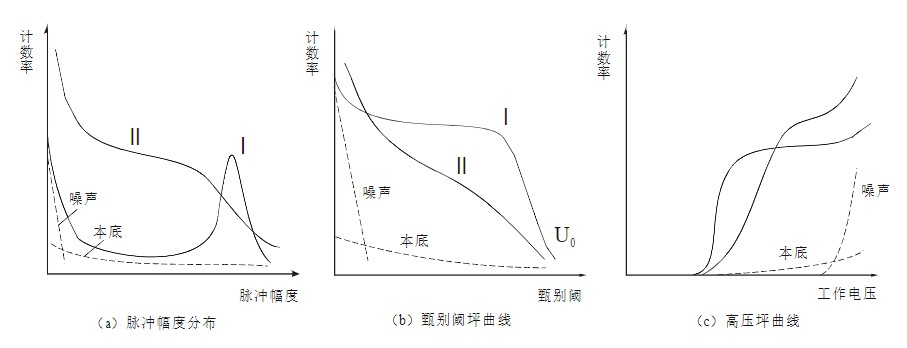
\includegraphics[width=0.9\textwidth]{./fig2.jpg}
        \caption{坪曲线与脉冲幅度谱的关系}
    \end{minipage}
\end{figure}

如果幅度分布谱为曲线I是单峰脉冲分布,相应的甄别阈曲线和高压坪曲线都将有一段坪区:
单峰区和低幅度高计数区之间的低计数区越长,坪越长;此区的计数越少,坪斜越小。

如果幅度分布谱为曲线II是连续脉冲分布,相应的甄别阈曲线和高压坪曲线都没有坪区。
$BF_3$正比计数管的脉冲分布谱决定了它的高压坪曲线和甄别阈曲线的形状。

\section{实验内容}

\begin{figure}[H]
    \centering
    \begin{minipage}[b]{0.9\textwidth}
        \centering
        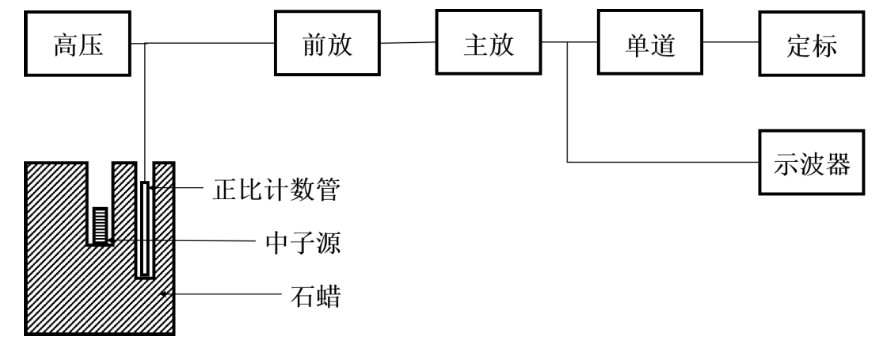
\includegraphics[width=0.9\textwidth]{./fig3.jpg}
        \caption{实验装置示意图}
    \end{minipage}
\end{figure}

用此套装置测量两条甄别阈—计数率曲线以及正比计数管的高压—计数率曲线。

\end{document}